\documentclass[10pt, a4paper]{article}

%%%%%%%%%%%%%%
%  Packages  %
%%%%%%%%%%%%%%


\usepackage{page_format}
\usepackage{special}
\usepackage{hyperref}
\usepackage{tikz}
\usepackage[compat=1.1.0]{tikz-feynman}
\input{math_func}

\usepackage{slashed}

% References
\usepackage{biblatex}
\addbibresource{ref.bib}


%%%%%%%%%%%%
%  Colors  %
%%%%%%%%%%%%
% ! EDIT HERE !
\colorlet{chaptercolor}{red!70!black} % Foreground color.
\colorlet{chaptercolorback}{red!10!white} % Background color

%%%%%%%%%%%%%%
% Page titre %
%%%%%%%%%%%%%%
\title{Homework 1} % Title of the assignement.
\author{\PA} % Your name(s).
\teacher{Francois David and Dan Wohns} % Your teacher's name.
\class{Quantum Field Theory II} % The class title.

\university{Perimeter Institute for Theoretical Physics} % University
\faculty{Perimeter Scholars International} % Faculty
%\departement{<Departement>} % Departement
\date{\today} % Date.


%%%%%%%%%%%%%%%%%%%%%%
% Begin the document %
%%%%%%%%%%%%%%%%%%%%%%
\begin{document}

% Make the title page.
\maketitlepage

% Make table of contents
\maketableofcontents

% Assignment starts here ----------------------------



\section{Gross-Neveu Model}

\begin{enumerate}
  \item[(a)] The Gross-Neveu model is a $1+1$ dimensionnal model describing a collection of $N$ fermionic fields $\psi^a$ (and a supressed Dirac index ranging from $1$ to $2$) indexed by a color index $a$ ranging from $1$ to $N$. The fermions each contribute a free massless Dirac term $\bar{\psi}_a i \slashed{\partial} \psi_a$ (summation on $a$ is implied) and are coupled with an interaction term $g^2 (\psi_a \psi^a)/(2N)$ with coupling constant $g$. The full lagrangian density reads
  \begin{align*}
    \mathcal{L}_{\mathrm{GN}}=\bar{\psi}_a i \slashed{\partial} \psi^a+\frac{g^2}{2 N}\left(\bar{\psi}_a \psi^a\right)^2. 
  \end{align*}
  We work in natural units where $\hbar = 1, c = 1$ making all quantitities of interest gain dimension of a power of mass. For action, length and time these powers are respectively $0$, $-1$ and $-1$. Since the action is dimensionless and obtained by integrating the lagrangian density $\mathcal{L}_{\mathrm{GN}}$ over $1+1$ spacetime dimensions, we have $0 = [\mathcal{L}_{\mathrm{GN}}] +  [dx^2] = [\mathcal{L}_{\mathrm{GN}}] - 2 \implies [\mathcal{L}_{\mathrm{GN}}] = 2$. Knowing the dimension of the lagrangian density, we use the kinetic term to compute the dimension of the fields. Since the derivatives have the inverse dimension of their associated variables, we have $2 = 2[\psi^a] + [\slashed{\partial}] = 2[\psi^a] + 1 \implies [\psi^a] = 1/2$. Finally, the dimension of the coupling constant can be extracted using the interaction term. Indeed,  $2 = 4 [\psi^a] + 2 [g] = 2 + 2 [g] \implies [g] = 0$ making the coupling constant dimensionless. 
  \item[(b)] The slashed derivative $\slashed{\partial}$ appearing in the lagrangian density is the result of a contraction of the $\gamma^\mu = (\gamma^0, \gamma^1)$ with the partial derivatives $\partial_\mu = (\partial_0, \partial_1)$. In $1+1$ dimensionnal spacetime we can form a clifford algebra with $\gamma^0 = \sigma^2, \gamma^1 = i \sigma^1$ where $\sigma^2, \sigma^1$ are Pauli matrices. We also have $\gamma^5 = \gamma^0 \gamma^1 = \sigma^3$. Following the properties of clifford algebras, we have that $\gamma^5$ anticommutes with all $\gamma^\mu$ matrices. All the $\gamma^\mu$ matrices are multiplied together in $\gamma^5$ and any $\gamma^\mu$ commutes with itself, but anticommutes with the remaining matrix in the product leading to $\{\gamma^5, \gamma^\mu\} = 0$. The Dirac adjoint of the fermionic fields appearing in the lagrangian density is defined to be $\bar{\psi}_a = \psi^{a\dagger} \gamma^0$.  We relate $\psi^{a}$ and a transformed field $\phi^{a}$ by $\psi^{a} = \gamma^5 \phi^{a}$. In terms of the transformed field, the  Dirac adjoint of $\psi^{a}$ becomes $\bar{\psi}_a = \phi^{a\dagger}\gamma^{5\dagger} \gamma^0 = -\phi^{a\dagger} \gamma^0 \gamma^{5} = -\bar{\phi}_a \gamma^5$ because $\gamma^5 = \sigma^3$ is real. Using these expressions, we can express $\mathcal{L}_{\mathrm{GN}}$ in terms of the transformed field as follows: 
  \begin{align*}
    \mathcal{L}_{\mathrm{GN}}=-\bar{\phi}_a \gamma^5 i \slashed{\partial} \gamma^5 \phi^a+\frac{g^2}{2 N}\left(-\bar{\phi}_a \gamma^5 \gamma^5 \phi^a\right)^2 = \bar{\phi}_a i \slashed{\partial}  \phi^a+\frac{g^2}{2 N}\left(\bar{\phi}_a \phi^a\right)^2  
  \end{align*}
  where we used $\{\gamma^5, \gamma^\mu\} = 0$ in the first term and $\gamma^5 = 1$ in the second term. We notice that the new lagrangian density is identical to the $\psi^a$ one and the transformation from $\psi^a$ to $\phi^a$ is a discrete symmetry. A mass $m$ term $m \bar{\psi}_a \psi^a$ would transform to $-m \bar{\phi}_a \gamma^5 \gamma^5 \phi^a = -m \bar{\phi}_a \phi^a$ which is not identical to the initial term and therefore breaks the considered symmetry. 
  \item[(c)] The interaction term implies that the scattering amplitudes can be computed using Feynman digragmatic for a $4$ particle vertex. Expanding the square of the interaction term we see that the vertex involves one (self-interaction) or two colors. For each color, it has an ingoing fermion and an outgoing fermion (arising from wick contractions with $\bar{\psi}_a$ and $\psi^a$). The coefficient of each color mixing term in the expansion is $g^2/N$ because the factor of $2$ is canceled by the binomial coefficient of the square expansion. The coefficient of single color terms is directly $g^2/(2N)$. We are interested in the two point function $\langle \bar{\psi}_b \psi_a\rangle$. At on loop order the only there is only one vertex and it has two of its fields contracted together to close the loop. Since non-vanishing contribtutions have contractions of equal color fields, the external fermions are requiered to be of the same (possibly different) color. The position space diagrams associated to this process and their amplitude are 
  \begin{equation*}
    \langle \bar{\psi}_a \psi_a \rangle_{\text{one \ loop}} = \dfrac{g^2}{N}\sum_{b\neq a}
    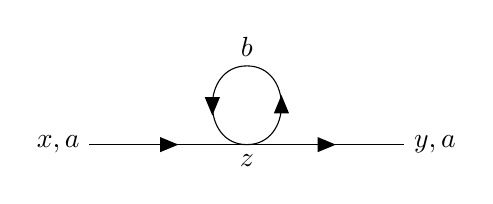
\begin{tikzpicture}[baseline=(current bounding box.center)]
      
      \begin{feynman}
        % External legs

        \vertex[label={left:$x, a$}]  (a) at (-2, 0);
        \vertex[label={right:$y, a$}] (b) at (2, 0);

        \vertex[label={below:$z$}]  (p) at (0, 0);
        \vertex[label={above:$b$}]  (q) at (0, 1);

        %\fill (a) circle (2pt);
  
        \diagram* {
          (a) --[fermion] (p),
          (p) --[fermion] (b),
          (p) --[fermion, half right] (q),
          (q) --[fermion, half right] (p),
        };
      \end{feynman}
    \end{tikzpicture}
    + 
    \dfrac{g^2}{2N}
    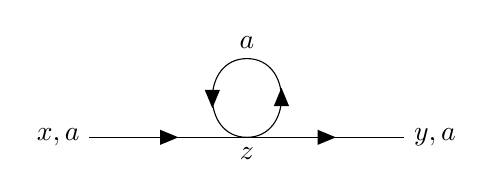
\begin{tikzpicture}[baseline=(current bounding box.center)]
      
      \begin{feynman}
        % External legs

        \vertex[label={left:$x, a$}]  (a) at (-2, 0);
        \vertex[label={right:$y, a$}] (b) at (2, 0);

        \vertex[label={below:$z$}]  (p) at (0, 0);
        \vertex[label={above:$a$}]  (q) at (0, 1);

        %\fill (a) circle (2pt);
  
        \diagram* {
          (a) --[fermion] (p),
          (p) --[fermion] (b),
          (p) --[fermion, half right] (q),
          (q) --[fermion, half right] (p),
        };
      \end{feynman}
    \end{tikzpicture}
  \end{equation*}
  \begin{equation*}
    = \frac{-ig^2}{\hbar N} (N-1) \int \ \text{d}^2 z \  \hbar (\slashed{\partial})^{-1}_{xz} \hbar (\slashed{\partial})^{-1}_{zz} \hbar (\slashed{\partial})^{-1}_{zy} + \frac{-ig^2}{2\hbar N}  \int \ \text{d}^2 z \  \hbar (\slashed{\partial})^{-1}_{xz} \hbar (\slashed{\partial})^{-1}_{zz} \hbar (\slashed{\partial})^{-1}_{zy}. 
  \end{equation*} 
  where $(\slashed{\partial})^{-1}_{xz}$ denotes the free massless fermionic propagator between points $x$ and $z$. We note that the amplitude takes the form of a matrix in spinor index consistently with the supressed spinor indices in $\langle \bar{\psi}_a \psi_a \rangle_{\text{one \ loop}}$.

  \item[(d)] We now consider an alternative theory involving a scalar field $\sigma(x)$ and the previously defined colored fermions $\psi^a$. The Lagrangian for this theory is
  \begin{align*}
    \mathcal{L}_{\psi, \sigma} = \bar{\psi}_a(i\slashed{\partial}-\sigma) \psi^a-\frac{N}{2 g^2} \sigma^2. 
  \end{align*} 
  In the Euclidean path integral formalism path the partition function of this theory is given by the following functionnal integral
  \begin{align*}
    Z = \int D[\sigma] \prod_{a} D[\bar{\psi}^a] D[\psi^a] \exp\left(\int \text{d}^2 z \ \mathcal{L}_{\psi, \sigma} \right)
  \end{align*} 
  with Grassman numbers as components of $\psi^a$ and their Grassman conjugate $(\psi^a)^\star$ apearing in the Dirac conjugate $\bar{\psi}^a = (\psi^a)^\star \gamma^0$. Integration in the exponential is performed on $\text{d}^2 z = -i\text{d}x \text{d}\tau$ with $\text{d}\tau = -i\text{d}t$ ($\tau = - i t$) the wick rotated time element. The Euclidean argument for the exponential derives from  
  \begin{align*}
    i \int_{M} \text{d} x \text{d} t  \ \mathcal{L}_{\psi, \sigma} \to  i(-i) \int_{\mathbb{R}^2} \text{d} x \text{d} \tau \ \mathcal{L}_{\psi, \sigma} = \int \text{d}^2 z \ \mathcal{L}_{\psi, \sigma} 
  \end{align*}
  where $M$ designates $(1, 1)$ Minkowski space and $\mathbb{R}^2$ designates Euclidean spacetime (which is implied in what follows). Since $\mathcal{L}_{\psi, \sigma}$ is a quadratic polynomial in $\sigma$ with negative coefficient for $\sigma^2$, the exponential forms a sequence of Gaussian integrals. By completing the square for this polynomial, we find 
  \begin{align*}
    Z &= \int D[\sigma] \prod_{a} D[\bar{\psi}^a] D[\psi^a] \exp\left(-\int \text{d}^2 z \ \frac{N}{2 g^2}\left(-i\frac{2 g^2}{N}\bar{\psi}_a\slashed{\partial}\psi^a+\frac{2 g^2}{N}\sigma \bar{\psi}_a \psi^a  + \sigma^2\right)\right)\\
    &=\int D[\sigma] \prod_{a} D[\bar{\psi}^a] D[\psi^a] \exp\left(-\int \text{d}^2 z \ \frac{N}{2 g^2}\left(-i\frac{2 g^2}{N}\bar{\psi}_a\slashed{\partial}\psi^a-\frac{2 g^4}{N^2} (\bar{\psi}_a \psi^a)^2  + \left(\sigma + \frac{g^2}{N} \bar{\psi}_a \psi^a\right)^2\right)\right)\\
    &= \prod_{a} D[\bar{\psi}^a] D[\psi^a] \int D\left[\sigma' - \frac{g^2}{N} \bar{\psi}_a \psi^a\right] \exp\left(-\int \text{d}^2 z \ \frac{N}{2 g^2}\left(-i\frac{2 g^2}{N}\bar{\psi}_a\slashed{\partial}\psi^a-\frac{g^4}{N^2} (\bar{\psi}_a \psi^a)^2  + \left(\sigma'\right)^2\right)\right)\\
    &= \left(\int D\left[\sigma'\right] \exp\left(- \int \text{d}^2 z\ \frac{N}{2g^2}(\sigma')^2\right) \right)  \int \prod_{a} D[\bar{\psi}^a] D[\psi^a]  \exp\left(-\int \text{d}^2 z \left(-i\bar{\psi}_a\slashed{\partial}\psi^a-\frac{g^2}{2N} (\bar{\psi}_a \psi^a)^2  \right)\right)\\
    &\sim \int \prod_{a} D[\bar{\psi}^a] D[\psi^a]  \exp\left(\int \text{d}^2 z\ \mathcal{L}_{GN}\right)
  \end{align*} 
  where the change of variable $\sigma' = \sigma + \frac{g^2}{N} \bar{\psi}_a \psi^a$ is associated to a trivial jaccobian because it consists in a shift. Since the numerical factor associated to the functionnal integral on $\sigma'$ is canceled when computing connected fermionic $n$-point functions, we conclude that the $\mathcal{L}_{\psi, \sigma}$ theory is equivalent to the $\mathcal{L}_{GN}$ theory when we are not concerned with $n$-point involving the scalar field. To treat them we would have to modify our analysis and include $\sigma$ source terms before defining $\sigma'$. 

  \item[(e)] We now perform the converse integration form the one done in (d). This time we aim to intergrate the fermionic degrees of freedom. We start with 
  \begin{align*}
    Z &= \int D[\sigma] \prod_{a} D[\bar{\psi}^a] D[\psi^a] \exp\left(\int \text{d}^2 z \ \bar{\psi}_a(i\slashed{\partial} - \sigma)\psi^a  - \frac{N}{2 g^2} \sigma^2\right)\\
    &= \int D[\sigma] \exp\left(- \int \text{d}^2 z\ \frac{N}{2g^2}\sigma^2\right) \prod_{a} D[\bar{\psi}^a] D[\psi^a] \exp\left(\int \text{d}^2 z \ \bar{\psi}_a(i\slashed{\partial} - \sigma)\psi^a\right).
  \end{align*}
  Then, we notice that the argument of the exponential in the fermionic functionnal integral can be expressed as a bilinear functionnal $F[\bar{\psi}_a, \psi^a] = \int \text{d}^2 z' \int \text{d}^2 z \bar{\psi}_a(z') \left[\delta(z-z') (i\slashed{\partial}_{z} - \sigma)\right] \psi^a (z)$. A generalisation of integration of Gaussians over grassman variable to functionnal analysis suggests that the result of the fermionic functionnal integral is the determinant of  $F[\bar{\psi}_a, \psi^a]$. This determinant is formaly written as the determinant of a matrix with continuous index $z, z'$ and elements at this index $\delta(z-z') (i\slashed{\partial}_{z} - \sigma)$. We denote this determinant with $\text{det}(\delta(z-z')(i\slashed{\partial}_{z} - \sigma))$. 
  \newpage
  Since the action involves $N$ decoupled colors, the determinant for one color functionnal integration is elevated to the power $N$ to represent the full integration. The properties of determinants allow us to write 
  \begin{align*}
    \text{det}(\delta(z-z')(i\slashed{\partial}_{z} - \sigma))^N &= \text{det}(\delta(z-z')(i\slashed{\partial}_{z} - \sigma))^N\\&=  \text{det}\left[ \exp(\text{log}(\delta(z-z')(i\slashed{\partial}_{z} - \sigma)))\right]^N\\&= \exp \left[\text{Tr}_{z, \text{spinor}}\left[\text{log}(\delta(z-z')(i\slashed{\partial}_{z} - \sigma))\right]\right]^N\\&= \exp \left[N \left[\int \text{d}^2 z \ \text{Tr}_{\text{spinor}}\text{log}(i  \slashed{\partial} - \sigma)_{zz}\right]\right].
  \end{align*}
  where $\text{log}(i  \slashed{\partial} - \sigma)_{zz}$ designates the $zz$ diagonal element of $\text{log}(\delta(z-z')(i\slashed{\partial}_{z} - \sigma))$. With this result, we have
  \begin{align*}
    Z &= \int D[\sigma] \exp\left(- \int \text{d}^2 z\ \frac{N}{2g^2}\sigma^2\right) \text{det}(\delta(z-z') (i\slashed{\partial}_{z} - \sigma))^N\\
    &= \int D[\sigma] \exp\left(\int \text{d}^2 z\ \left(-\frac{N}{2g^2}\sigma^2 + N \text{Tr}_{\text{spinor}}\text{log}(i  \slashed{\partial} - \sigma)_{zz}\right)\right).  
  \end{align*}
  \item[(f)] Taking the number of colors to infinity allows to evalutate approximatly the last functionnal integral using a saddle-point approximation. The saddle point configuration is associated to the field extremizing the eclidean action
  \begin{align*}
    S[\sigma] = -\int \text{d}^2 z\ \left(-\frac{N}{2g^2}\sigma^2 + N \text{Tr}_{\text{spinor}}\text{log}(i  \slashed{\partial} - \sigma)_{zz}\right)
  \end{align*}
  with respect to $\sigma$. Assuming the saddle point field is a constant $\phi_c$, we find that 
  We can find this configuration by considering a small deformation field $\delta \phi$. The saddle-point field is such that this variation leaves the action invariant at first order in $\delta \phi$. Up to first order, we have 
  \begin{align*}
    S[\sigma_c + \delta \phi] = -\int \text{d}^2 z\ \left[-\frac{N}{2g^2}\sigma_c^2 - \frac{N}{g^2} \sigma_c \delta\sigma + N \text{Tr}_{\text{spinor}}\text{log}(i  \slashed{\partial} - \sigma_c)_{zz} + N \delta\sigma\left.\frac{\partial}{\partial \sigma}\right|_{\sigma = \sigma_c} \text{Tr}_{\text{spinor}}\text{log}(i  \slashed{\partial} - \sigma_c)_{zz}\right].
  \end{align*} 
  In order to evaluate the derivative of the trace term, a UV regulator $\Lambda$ is introduced to write 
  \begin{align*}
    \left.\frac{\partial}{\partial \sigma}\right|_{\sigma = \sigma_c} \text{Tr}_{\text{spinor}}\text{log}(i  \slashed{\partial} - \sigma_c)_{zz} = \frac{\sigma_c}{4 \pi} \log \left(\frac{\Lambda^2}{\sigma_c^2}\right).
  \end{align*}
  With this result, the first order variation of the action reads
  \begin{align*}
     \delta S = -\int \text{d}^2 z\ \left[ - \frac{N}{g^2} \sigma_c + N \frac{\sigma_c}{4 \pi} \log \left(\frac{\Lambda^2}{\sigma_c^2}\right)\right] \delta\sigma.
  \end{align*} 
  Since $\delta \sigma$ is arbitrary, we have the saddle-point condition 
  \begin{align*}
    0 = - \frac{N}{g^2} \sigma_c + \sigma_c \frac{N}{4 \pi} \log \left(\frac{\Lambda^2}{\sigma_c^2}\right) \iff \sigma_c = \pm\Lambda e^{-2\pi/g^2} \quad  \text{or} \quad \sigma_c \to 0 \quad (\text{the limit exists}).
  \end{align*}
  We notice that the argument of the exponential is dimensionless because $g$ is dimensionless as shown in (a). It remains to confirm if these solutions are saddle-points are extrema of minima. To do it, we write the second order variation of $S$ as follows:
  \begin{align*}
    \delta^2 S = -\int \text{d}^2 z\ \left[-\frac{N}{2g^2} + \frac{N}{4 \pi} \log \left(\frac{\Lambda^2}{\sigma_c^2}\right) - \frac{N}{4 \pi} \frac{\sigma_c^3}{\Lambda^2} \frac{\Lambda^2}{2 \sigma_c^3} \right] \delta \sigma^2 = -\int \text{d}^2 z\ \left[-\frac{N}{2g^2} - \frac{N}{8 \pi} - \frac{N}{4 \pi} \log \left(\frac{\sigma_c^2}{\Lambda^2}\right) \right] \delta \sigma^2
  \end{align*}
  for $\phi_c = \pm\Lambda e^{-2\pi/g^2}$ we get an integrand of $\frac{N}{2g^2} + \frac{N}{8 \pi} - \frac{N}{2 g^2} = + \frac{N}{8 \pi}$ (Minimum, but the $-$ saddle-point would lead to negative mass and instability breaking our hypothesis of $\phi_c$ being constant). For $\phi_c \to 0$, we have a negative diverging integrand (Maximum). The relevant saddle-point here is therefore $\phi_c = \Lambda e^{-2\pi/g^2}$. (This analysis seems to be incomplete, and a more detailed stability treatement could help make the choice of saddle-point more meaningful). 
  \item[(g)] Taking $\phi_c = \Lambda e^{-2\pi/g^2}$ in the limit $N \to \infty$, the $\mathcal{L}_{\psi, \sigma}$ theory (equivalent to the $\mathcal{L}_{GN}$ theory by (d)) becomes a theory with non-dynamical $\sigma$ that gains the interpretation of the mass of the colored fermions. Indeed, $\sigma$ plays the role of a mass term in $\bar{\psi}_a(i\slashed{\partial}-\sigma) \psi^a$ and this seems to break the chiral symmetry of the $\mathcal{L}_{GN}$. Performing the steps of the scalar field functionnal integral of question (d) in reverse seems to suggest that extra couplings can emerge from functionnal integration itself. Finally, we notice that the effective mass depends on a scale $\Lambda$ while the initial theory has $g$ dimensionless (providing no natural scale). This implies that the introduction of the UV regulator is the source of chiral symmetry breaking because it is not consistent with our initial set of parameters.  
\end{enumerate}



\section{Acknowledgement}

Thanks to Maitá and Thomas for pointing out that the one-loop diagrams with loops differently colored from external points do not vanish. 

Thanks to Nikhil and Jaroslav for discussions about the role of a bilinear functionnal in the interpretation of a functionnal determinant. 

Thanks to Jaroslav for his PSIminar about anolmalies giving me a starting point in the study of anomalies. 

Thanks to Hyo Jung for a discussion about the implications of the presence of a coupling in the effective mass. 




% References
\makereferences
%-------------------------------------------------------


%%%%%%%%%%%%%%%%%%%%%%%%
% Terminer le document %
%%%%%%%%%%%%%%%%%%%%%%%%
\end{document}
